\documentclass[unicode, notheorems]{beamer}
\usepackage{graphicx}
% If you have more than three sections or more than three subsections in at least one section,
% you might want to use the [compress] switch. In this case, only the current (sub-) section
% is displayed in the header and not the full overview.
\mode<presentation>
{
  \usetheme[numbers, totalnumbers, minimal]{Statmod}

\setbeamercovered{transparent}
  % or whatever (possibly just delete it)
{\tiny }}
\setbeamercolor{alerted text}{fg=blue}

%\usepackage{pscyr}
\usepackage[T2A]{fontenc}
\usepackage[cp1251]{inputenc}
\usepackage[russian]{babel}
\usepackage{amsthm}

%\usepackage{tikz}
% you only need this when using TikZ graphics

\newtheorem{theorem}{Утверждение}
\newtheorem{example}{Пример}
\newtheorem{definition}{Определение}
\newtheorem{task}{Задача}
\newtheorem{def1}{Определение}
\newtheorem{proposition}{Утверждение}
\newtheorem{notice}{Замечание}
\newtheorem{task_regul}{Задача с регуляризацией}
\DeclareMathOperator{\sign}{sign}
\DeclareMathOperator*{\argmax}{arg\,max} 

\title[Обучение с учителем. Классификация]{Обучение с учителем. Классификация. Функция риска. Логистическая регрессия. Feature selection и extraction}

\author[А.Третьякова, М.Волканова, Н.Федоров]{Третьякова Александра Леонидовна, \\ Волканова Маргарита Дмитриевна, \\
	 Федоров Никита Алексеевич}

\date{
    Санкт-Петербург\\
    2019г.
}

\subject{Beamer}
% This is only inserted into the PDF information catalog. Can be left
% out.

% Delete this, if you do not want the table of contents to pop up at
% the beginning of each subsection:
% \AtBeginSubsection[]
% {
%   \begin{frame}<beamer>
%     \frametitle{Outline}
%     \tableofcontents[currentsection,currentsubsection]
%   \end{frame}
% }

\begin{document}

\begin{frame}
    \titlepage
\end{frame}


\begin{frame}
    \frametitle{Обучение с учителем. Постановка задачи}
 $\mathsf{X}$ --- множество объектов, $\mathsf{Y}$ --- множество ответов \\
 $\mathsf{y}: \mathsf{X}\to \mathsf{Y}$ --- неизвестная зависимость (target function) \\
 ~\\
 Дано: обучающая выборка --- $\mathsf{(x_1,\ldots, x_n) \subset X}$, $\mathsf{y_i=y(x_i), ~i=1,\ldots,n}$ --- известные ответы. \\
 Найти: $\mathsf{a:X\to Y}$ --- функцию (decision function), приближающую $\mathsf{y}$ на всем множестве $\mathsf{X}$. \\
   ~\\
 Вероятностная постановка задачи: имеется неизвестное распределение на множестве $\mathsf{X\times Y}$ с плотностью $\mathsf{p(x,y)}$, из которого случайно выбираются $\mathbb{X}_\mathsf{n}=\mathsf{(x_i,y_i)_{i=1}^n}$ (независимые). \\
  ~\\
 Задача классификации: 
 \begin{itemize}
 	\item $\mathsf{Y}=\{-1,+1\}$ --- классификация на 2 класса
 	\item $\mathsf{Y}=\{1,\ldots,K\}$ --- классификация на $K$ классов
 \end{itemize}
\end{frame}

\begin{frame}
\frametitle{Обучение с учителем. Постановка задачи}
Обучающая выборка: $\mathbb{X}_\mathsf{n}=\mathsf{(x_i,y_i)_{i=1}^n},~\mathsf{x_i}\in \mathbb{R}^\mathsf{p},~ \mathsf{y_i}\in \{-1,+1\}.$
$\mathsf{f(x,w)}$ --- разделяющая (дискриминантная) функция, $\mathsf{w}\in\mathbb{R}^\mathsf{p}$. \\

$\mathsf{a(x,w)=\sign f(x,w)}$ --- классификатор. \\

$\mathsf{f(x,w)}=0$ --- разделяющая поверхность. \\
~~\\

$\mathsf{M_i(w)=y_if(x_i,w)}$ --- \alert{отступ} объекта $\mathsf{x_i}$. 

Если $\mathsf{M_i(w)<0},$ то классификатор ошибается на $\mathsf{x_i}$.
\begin{task}
	$Q(\mathsf{w)=\sum \limits_{i=1}^n \alert{[M_i(w)<0]}}\le \tilde Q(\mathsf{w)=\sum \limits_{i=1}^n \alert{\mathcal{L}(M_i(w))} \to \min \limits_{w}}$
\end{task}
%\alert{Метод:} метод стохастического градиента.
\begin{figure}[h]
	\begin{center}
		\begin{minipage}[h]{0.55\linewidth}
			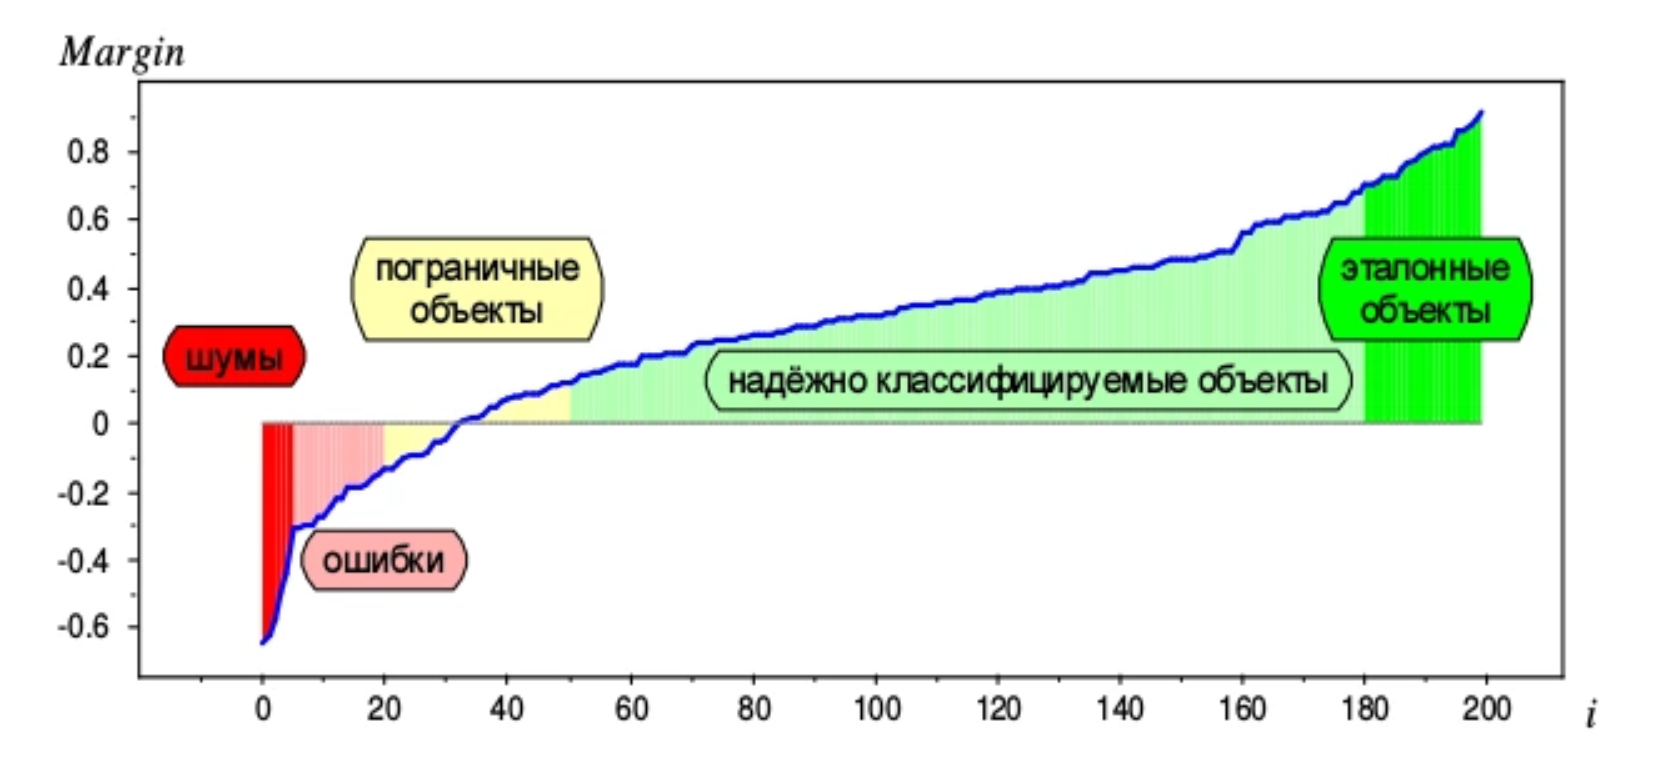
\includegraphics[width=1\linewidth]{Margins}
			\caption{}
			\label{series_IRLS} %% метка рисунка для ссылки на него
		\end{minipage}
	\end{center}
\end{figure}
\end{frame}

\begin{frame}
	\frametitle{Примеры функции потерь}
	\begin{itemize}
	\item \alert{Пороговая функция потерь: $\mathsf{[M_i(w)<0]}$}\\
	\item Логарифмическая: $\mathsf{\log_2 (1+e^{-M_i(w)})}$  \\
	\item Экспоненциальная: $\mathsf{e^{-M_i(w)}}$  \\
	\item Кусочно-линейная: $\mathsf{(1-M_i(w))_{+}}$ \\
	\item Квадратичная: $\mathsf{(1-M_i(w))^2}$ 

	 \end{itemize}
\begin{figure}[h]
	\begin{center}
		\begin{minipage}[h]{0.555\linewidth}
			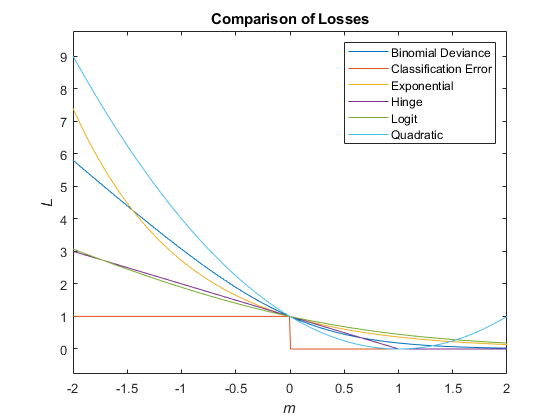
\includegraphics[width=1\linewidth]{lossfunc}
			\caption{Примеры функции потерь $\mathcal{L}(M)$}
			\label{series_IRLS} %% метка рисунка для ссылки на него
		\end{minipage}
	\end{center}
\end{figure}

\end{frame}


\begin{frame}
    \frametitle{Линейный классификатор}
$\mathsf{f_j:X\to\mathbb{R},~j=1,\ldots,p}$
 
 Линейная модель классификации: 
 \begin{equation*}
 \mathsf{a(x,w)=\sign (\sum\limits_{j=1}^pw_jf_j(x)-w_0),~~~w_0,w_1,\ldots,w_p\in\mathbb{R}}.
 \end{equation*}
 Пусть $\mathsf{f_0=-1}$, тогда
 \begin{equation*}
 \mathsf{a(x,w)=\sign\langle w,x\rangle ,~ x,w\in\mathbb{R}^{p+1}}.
 \end{equation*} 
 
 $\mathsf{M_i(x)=y_i\langle w,x_i\rangle}$ --- отступ объекта $\mathsf{x_i}$. 
 
 \begin{task}
 		$\mathsf{Q(w)=\sum \limits_{i=1}^n [y_i\langle w,x_i\rangle <0] \le \sum \limits_{i=1}^n \mathcal{L}(y_i\langle w,x_i\rangle) \to \min \limits_{w}}$
 \end{task}

Проверка по тестовой выборке $\tilde{\mathbb{X}}_\mathsf{k}=\mathsf{(\tilde{x}_i,\tilde{y}_i)_{i=1}^k}$:
\begin{equation*}
\mathsf{\bar{Q}(w)=\frac{1}{k}\sum\limits_{i=1}^k [\tilde{y}_i\langle w,\tilde{x}_i\rangle <0]}
\end{equation*}
\end{frame}

\begin{frame}
\frametitle{Решение задачи оптимизации}
Для решения задачи оптимизации используется \\ \alert{метод стохастического градиента}. \\
~\\
Вход: $\mathbb{X}_\mathsf{n}=\mathsf{(x_i,y_i)_{i=1}^n, h, \lambda}$ \\
Выход: $\mathsf{w}$
\begin{enumerate}
	\item Инициализация $\mathsf{w_j,~ j=0,\ldots,p}$ \\
	\item Инициализация $\mathsf{\bar{Q}(w)}$ \\
	\item {Повторять
		\begin{enumerate}
			\item Выбор $\mathsf{x_i}$ из $\mathbb{X}_\mathsf{n}$ случайным образом \\
			\item Вычисление $\mathsf{\varepsilon_i := \mathcal{L}_i(w)}$ \\
			\item Градиентный шаг $\mathsf{w:=w-h\nabla\mathcal{L}_i(w) }$ \\
			\item Вычисление $\mathsf{\bar{Q}(w):=\lambda\varepsilon_i+(1-\lambda)\bar{Q}(w)}$ \\
		\end{enumerate} 
	пока $\mathsf{\bar{Q}(w)}$ или $\mathsf{w}$ не сойдутся
	}
\end{enumerate}


\end{frame}
%\begin{frame}
%    \frametitle{Using Ti\textit{k}Z for Drawings}

    % The stuff for this slide is taken from the PGF Manual

 %   \begin{tikzpicture}
 %      \draw[fill=yellow] (0,0) -- (60:.75cm) arc (60:180:.75cm);
 %       \draw(120:0.4cm) node {$\alpha$};
 %       \draw[fill=green!30] (0,0) -- (right:.75cm) arc (0:60:.75cm);
 %       \draw(30:0.5cm) node {$\beta$};
 %       \begin{scope}[shift={(60:2cm)}]
%            \draw[fill=green!30] (0,0) -- (180:.75cm) arc (180:240:.75cm);
 %           \draw (30:-0.5cm) node {$\gamma$};
 %           \draw[fill=yellow] (0,0) -- (240:.75cm) arc (240:360:.75cm);
%            \draw (-60:0.4cm) node {$\delta$};
 %       \end{scope}
 %       \begin{scope}[thick]
  %          \draw (60:-1cm) node[fill=red!20] {$E$} -- (60:3cm) node[fill=red!20] {$F$};
 %           \draw[red] (-2,0) node[left] {$A$} -- (3,0) node[right]{$B$};
 %           \draw[blue,shift={(60:2cm)}] (-3,0) node[left] {$C$} -- (2,0) node[right]{$D$};
 %       \end{scope}
 %       \path (5,-0.5) node (x) {Hello World!}
 %       (7.5,2) node[circle,draw](y) {$\int_1^2 x \mathrm d x$};
 %       \draw[->,blue] (x) -- (y);
 %       \draw[->,red] (x) -| node[near start,below] {\footnotesize Red} (y);
 %       \draw[->,orange] (x) .. controls +(up:1cm) and +(left:1cm) .. node[above,sloped] {\footnotesize Orange} (y);
 %   \end{tikzpicture}
%
%  \vspace*{.5cm}
%
%  Take a look into the \alert{souce code} to see how this is done.
%
%\end{frame}

\begin{frame}
	\frametitle{Регуляризация}
\alert{Проблемы:}
\begin{itemize}
\item Признаков намного больше, чем объектов
\item {Мультиколлинеарность признаков: \\
%	Пусть $\exists u\in \mathbb{R}^{n+1}:<u,x>=0,$ тогда $\forall \gamma\in\mathbb{R}~ a(x,w)=\sign <w+\gamma u,x>$ (алгоритм выдает любое из семейства решений, $\Arrowvert w \Arrowvert$ может быть большой).
Пусть $\mathsf{a(x,w)=\sign (w_1f_1(x)+w_2f_2(x)-w_0),~~ f_2(x)=kf_1(x)}$. \\
Тогда $\mathsf{w_1f_1(x)+w_2f_2(x)=(w_1+\beta)f_1(x)+(w_2-k\beta)f_2(x)~ \forall \beta}$}
\end{itemize}
Таким образом, очень много различных векторов дадут близкие значения функционала качества, но при этом коэффициенты могут существенно отличаться. Признаком такого явления может являться большая $\Arrowvert \mathsf{w} \Arrowvert$. 
\begin{task_regul}
	$Q(\mathsf{w},\mathbb{X}_\mathsf{n})=Q(\mathsf{w},\mathbb{X}_\mathsf{n})+\frac{\tau}{2}\Arrowvert \mathsf{w} \Arrowvert ^2 \to \min \limits_\mathsf{w}$
\end{task_regul}	

\end{frame}

\begin{frame}
	\frametitle{Связь с принципом максимума правдоподобия}
	Рассмотрим \alert{модель}: пусть $\mathsf{X\times Y}$ --- вероятностное пространство с плотностью $\mathsf{p(x,y|w)}$.
	
	Пусть $\mathbb{X}_\mathsf{n}=\mathsf{(x_i,y_i)_{i=1}^n \sim p(x,y|w)}$ --- независимы, одинаково распределены. 
	\begin{itemize}
		\item {\alert{Максимизация правдоподобия:}\\
		$L(\mathsf{w};\mathbb{X}_\mathsf{n})=\ln\prod\limits_{i=1}^n \mathsf{p(x_i,y_i|w)}=\sum\limits_{i=1}^n \ln \mathsf{p(x_i,y_i|w) \to \max\limits_w}$.}
		
		\item {\alert{Минимизация аппроксимированного эмпирического риска:}\\
			$\tilde{Q}(\mathsf{w};\mathbb{X}_\mathsf{n})=\sum\limits_{i=1}^n \mathcal{L}(\mathsf{y_if(x_i,w)) \to \min\limits_w}$.}
		
	\end{itemize}
Эти задачи эквивалентны, если положить $-\ln \mathsf{p(x_i,y_i|w)} = \mathcal{L}(\mathsf{y_if(x_i,w)})$. \\
~~\\
\alert{Пример:}
$\mathsf{p(x,y|w)}=\frac{1}{1+\exp(- y\langle x,w \rangle )}$ (сигмоидная функция), ~ $\mathsf{\mathcal{L}(yf(x,w))=\log (1+exp(-y\langle x,w \rangle))}$ (логарифмическая функция потерь)
\end{frame}

\begin{frame}
	\frametitle{Связь с принципом максимума правдоподобия}
	\alert{Модель}: $\mathbb{X}_\mathsf{n}=\mathsf{(x_i,y_i)_{i=1}^n \sim p(x,y|w)}$ --- н.о.р.,
	
	Пусть $\mathsf{w\sim p(w;\gamma)}$, $\mathsf{\gamma}$ --- вектор гиперпараметров. Тогда: 
	\begin{equation*}
	\mathsf{p}(\mathbb{X}_\mathsf{n},\mathsf{w)=p(\mathbb{X}_n|w)p(w;\gamma)}
	\end{equation*}
	Принцип максимума правдоподобия:
		\begin{equation*}
    L(w;\mathbb{X}_\mathsf{n})=\ln \mathsf{p(\mathbb{X}_n,w)=\sum\limits_{i=1}^n p(x_i,y_i|w)+\underbrace{\ln p(w;\gamma)}_{\text{регуляризатор}} \to \max\limits_{w,\gamma}}
	\end{equation*}
\alert{Примеры:} \begin{enumerate}
	\item {\alert{Гауссовский регуляризатор}: $\mathsf{p(w;\sigma)=\frac{1}{(2\pi\sigma)^{p/2}}\exp{-\frac{\Arrowvert w \Arrowvert ^2}{2\sigma}}}$,\\
		тогда $-\ln \mathsf{p(w;\sigma)=\frac{1}{2\sigma}\Arrowvert w \Arrowvert ^2+\text{const}~~(\tau=1/\sigma)}$}
	\item {\alert{Регуляризатор Лапласа} (приводит к отбору признаков): $\mathsf{p(w;C)=\frac{1}{(2C)^{p}}\exp{-\frac{\Arrowvert w \Arrowvert _1}{C}}}$,\\
		тогда $-\ln \mathsf{p(w;C)=\frac{1}{C}\sum\limits_{j=1}^p|w_j|+\text{const}~~(\tau=1/C)}$}
\end{enumerate}
\end{frame}


\begin{frame}
	\frametitle{Регуляризатор Лапласа. Отбор признаков}
Задача: $Q(\mathsf{w;\mathbb{X}_n)=\sum\limits_{i=1}^n \ln p(x_i,y_i|w)+\frac{1}{C}\sum\limits_{j=1}^p|w_j| \to \min\limits_{w,C}}$.

Замена: $\begin{cases} \mathsf{u_j=\frac{1}{2}(|w_j|+w_j)} \\ \mathsf{v_j=\frac{1}{2}(|w_j|-w_j)} \end{cases}$, тогда $\begin{cases} \mathsf{w_j=u_j-v_j} \\ \mathsf{|w_j|=u_j+v_j} \end{cases}$,

\begin{equation*}
\begin{cases}
Q(\mathsf{u,v)=\sum \limits_{i=1}^n \mathcal{L}(M_i(u-v,w_0))+\frac{1}{C}\sum\limits_{j=1}^p (u_j+v_j) \to \min\limits_{u,v}} \\
\mathsf{u_j\ge 0,~v_j\ge 0,~~ j=1,\ldots,p}
\end{cases}
\end{equation*}
При уменьшении $\mathsf{C}$ (возрастании $\mathsf{\frac{1}{C}}$) обнуляются $\mathsf{u_j}$ и $\mathsf{v_j}$ для все большего количества $\mathsf{j}$, то есть $\mathsf{w_j=0}$ и признак не учитывается. 

При $\mathsf{C\to 0}$ выбросим все признаки.
\end{frame}

\begin{frame}
\frametitle{Логистическая регрессия. Подход через минимизацию функции потерь}
Линейная модель классификации: $\mathsf{a(x)=\sign \langle w,x\rangle,~~ x,w\in \mathbb{R}^p,~~ M=\langle w,x \rangle y}$ --- отступ. \\
~~\\

В качестве аппроксимации пороговой функции потерь берется логарифмическая функция потерь $\mathcal{L}(\mathsf{M})=\log(1+e^{-\mathsf{M}}).$ \\
%\begin{task}
%	$\mathsf{Q(w)=\sum \limits_{i=1}^n (1+\exp{(-y_i\langle w,x_i\rangle)}) \to \min \limits_{w}}$
%\end{task}

\begin{figure}[h]
	\begin{minipage}[h]{0.6\linewidth}
		\center{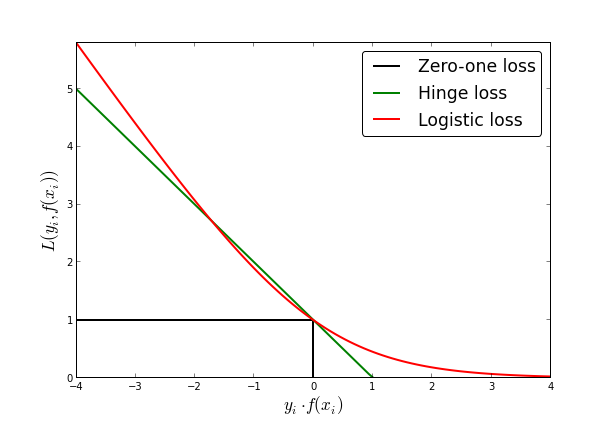
\includegraphics[width=0.9\linewidth]{loss_function}}
	\end{minipage}
	%\caption{Зависимость сигнала от шума для данных.}
	\label{ris:image1}
\end{figure}
\end{frame}

\begin{frame}
\frametitle{Логистическая регрессия. Подход через минимизацию функции потерь}

\begin{task}
	$\mathsf{Q(w)=\sum \limits_{i=1}^n \log (1+\exp{(-y_i\langle w,x_i\rangle)}) \to \min \limits_{w}}$
\end{task}

Методы решения задачи минимизации:
\begin{itemize}
	\item метод стохастического градиента
	\item метод Ньютона-Рафсона
\end{itemize}
\end{frame}

\begin{frame}
\frametitle{Логистическая регрессия. Вероятностный подход}
%Методы решения задачи минимизации: метод стохастического градиента, метод Ньютона-Рафсона. \\
~~\\

$\mathsf{P(y|x,w)=\sigma_w(M)=\frac{1}{1+e^{-\langle x,w \rangle y}}}$ --- сигмоидная функция.

Свойства $\mathsf{\sigma(z)}$:
\begin{itemize}
	\item $\mathsf{\sigma(z)} \in [0,1]$ , задана на $(-\infty,+\infty)$ \\
	\item {$\mathsf{\sigma(z)\to 1,~ z\to +\infty};$ \\ $\mathsf{\sigma(z)\to 0,~ z\to -\infty} $} \\
	\item $\mathsf{\sigma(z)+\sigma(-z)=1}$ \\
	\item $\mathsf{\sigma ' (z)=\sigma (z)\sigma(-z)}$ \\
	%\item {$\mathsf{\sigma(z)\ge 0.5}$ при $\mathsf{z\ge 0}$ \\
	%$\mathsf{\sigma(z)< 0.5}$ при $\mathsf{z< 0}$}
\end{itemize}

\begin{figure}[h]
	\begin{center}
		\begin{minipage}[h]{0.4\linewidth}
			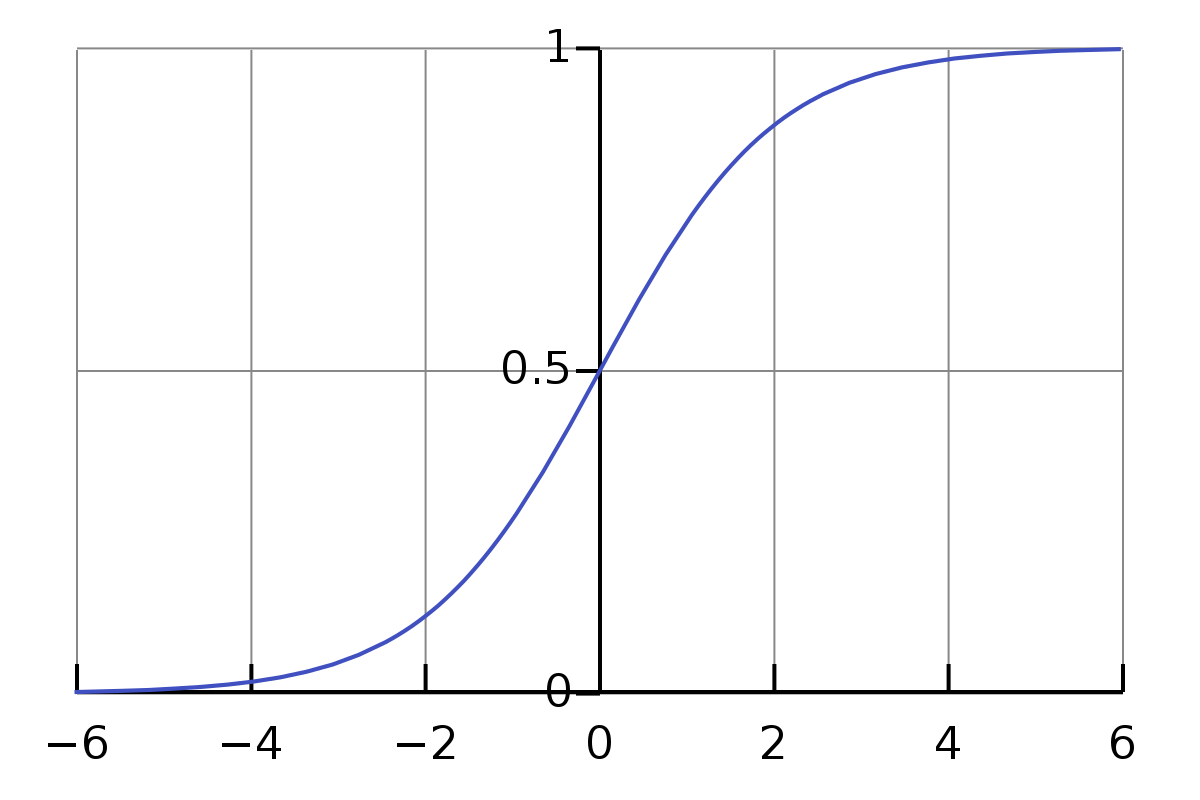
\includegraphics[width=1\linewidth]{sigmoid2}
			\caption{Сигмоидная функция}
			\label{series_IRLS} %% метка рисунка для ссылки на него
		\end{minipage}
		
	\end{center}
\end{figure}
\end{frame}

\begin{frame}
\frametitle{Логистическая регрессия. Вероятностный подход}
Пусть $\mathsf{Y}=\{0,1\}$. \\
\begin{itemize}
	\item $\mathsf{P(y_i=1|x;w)=\sigma_w(x)}$ \\
	\item $\mathsf{P(y_i=0|x;w)=1-\sigma_w(x)}$ \\
\end{itemize}
Тогда $\mathsf{P(y|x;w)=(\sigma_w(x))^y(1-\sigma_w(x))^{1-y}}.$ \\
Функция правдоподобия:
\begin{equation*}
\mathsf{Q(w)=-\log L(w)=-\log \prod\limits_{i=1}^n(\sigma_w(x_i))^{y_i}(1-\sigma_w(x_i))^{1-y_i}}= 
\end{equation*}
\begin{equation*}
=\mathsf{-\sum\limits_{i=1}^n [y_i\log (\sigma_w(x_i)+(1-y_i))\log (1-\sigma_w(x_i))]\to \min\limits_{w}}
\end{equation*}
\begin{figure}[h]
	\begin{center}
		\begin{minipage}[h]{0.7\linewidth}
			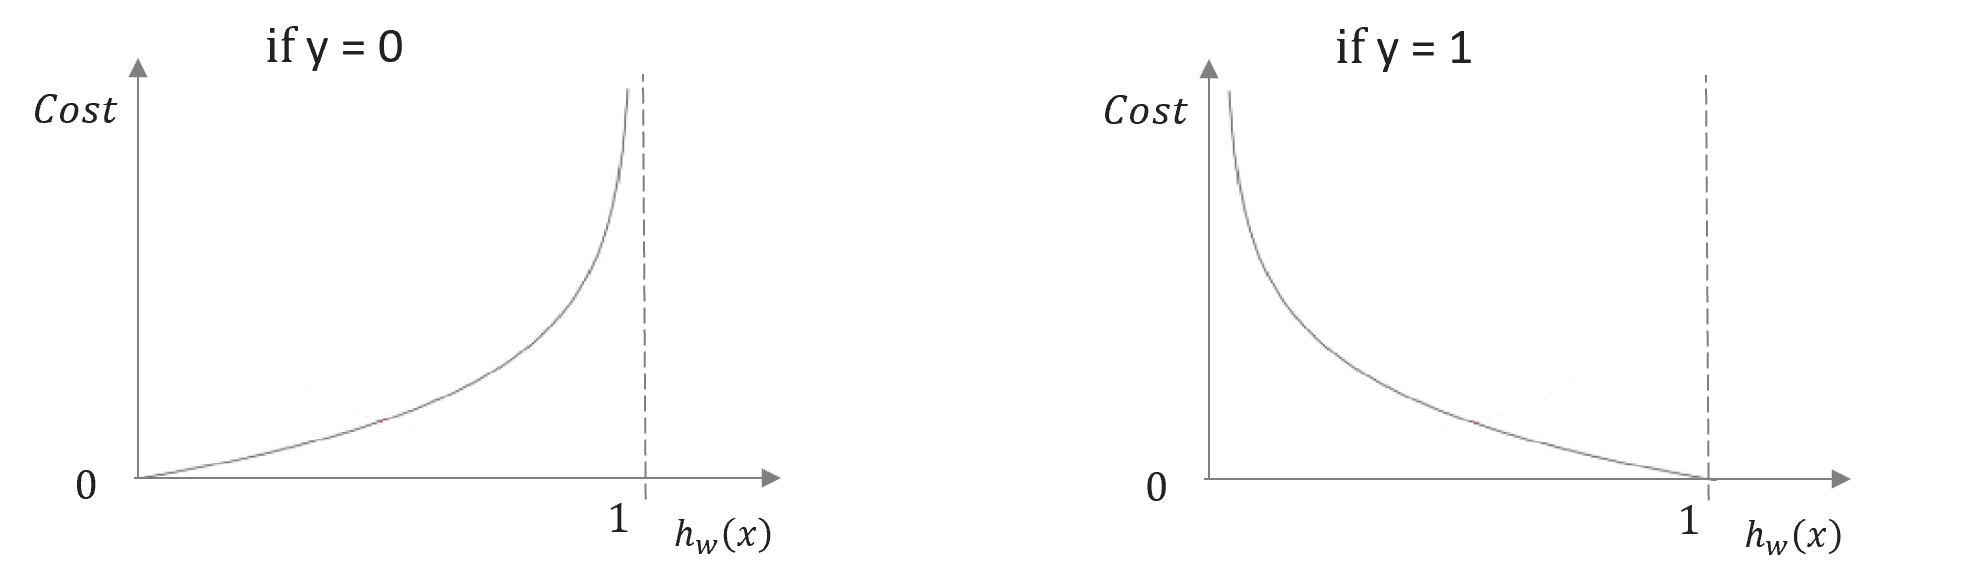
\includegraphics[width=1.2\linewidth]{cost}
			%\caption{}
			\label{series_IRLS} %% метка рисунка для ссылки на него
		\end{minipage}
		
	\end{center}
\end{figure}
\end{frame}


\begin{frame}
\frametitle{Линейная и логистическая регрессия}

\begin{figure}[h]
	\begin{center}
		\begin{minipage}[h]{0.6\linewidth}
			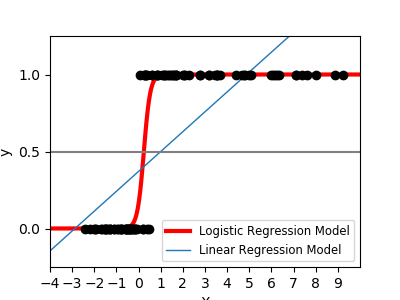
\includegraphics[width=1\linewidth]{regression}
			\caption{Линейная и логистическая регрессия}
			\label{series_IRLS} %% метка рисунка для ссылки на него
		\end{minipage}
	
	\end{center}
\end{figure}
\end{frame}



\begin{frame}
\frametitle{Логистическая регрессия. Регуляризация}
$\mathsf{Q(w)=-\sum\limits_{i=1}^n [y_i\log (\sigma_w(x_i)+(1-y_i))\log (1-\sigma_w(x_i))]}$ \\
~~\\
Регуляризация в логистической регрессии:
\begin{itemize}
	\item {\alert{L2}: 
	$\mathsf{Q_\tau(w)=Q(w)+\frac{\tau}{2}\sum\limits_{j=1}^p w_j^2 \to \min\limits_w}$
		}
	\item {\alert{L1}: 
		$\mathsf{Q_\tau(w)=Q(w)+\tau\sum\limits_{j=1}^p |w_j| \to \min\limits_w}$
	}
\end{itemize}
Параметр $\mathsf{\tau}$ можно подбирать с помощью кросс-валидации. \\
~ \\
Методы решения задачи минимизации: метод стохастического градиента, метод Ньютона-Рафсона.
\end{frame}

	
	\begin{frame}
	\frametitle{Логистическая регрессия. Добавление нелинейных признаков}
	Можно ли использовать логистическую регрессию в случае, когда нет линейной разделимости?
	\begin{figure}[h]
		\begin{center}
			\begin{minipage}[h]{0.75\linewidth}
				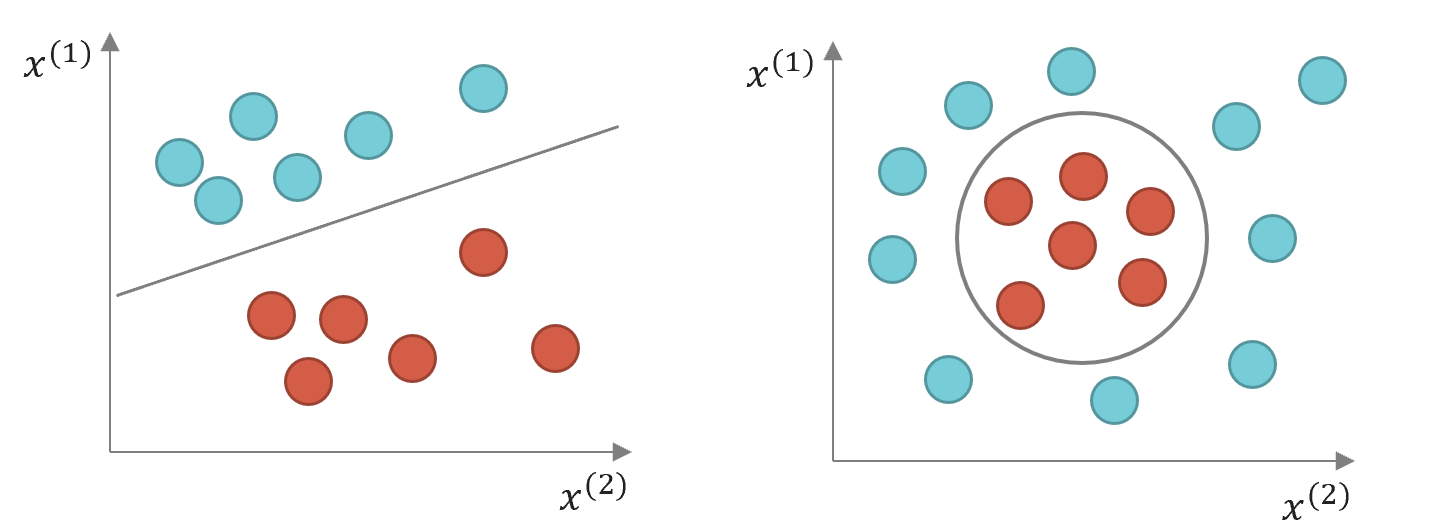
\includegraphics[width=1\linewidth]{nonlinear}
				%\caption{Линейная и логистическая регрессия}
				\label{series_IRLS} %% метка рисунка для ссылки на него
			\end{minipage}
			
		\end{center}
	\end{figure}
\begin{minipage}{0.5\textwidth}
	$\mathsf{\langle w,x\rangle =w_1x_1+w_2x_2+w_0}$ \\
	Разделяющая поверхность: \\
	$\mathsf{w_1x_1+w_2x_2+w_0 =0}$
\end{minipage}
\hfill
\begin{minipage}{0.45\textwidth}
	$\mathsf{\langle w,x\rangle =w_1x_1^2+w_2x_2^2+w_0}$ \\
Разделяющая поверхность: \\
$\mathsf{w_1x_1^2+w_2x_2^2+w_0 =0}$
\end{minipage}
\end{frame}


\begin{frame}
	\frametitle{Многоклассовая логистическая регрессия}
	Линейный классификатор при произвольном числе классов $\mathsf{Y=\{1,\ldots,K\}}$: 
	\begin{equation*}
	\mathsf{a(x,w)=\argmax_{y\in Y}\langle w_y,x \rangle,~~~x,w_y\in\mathbb{R}^p }
	\end{equation*}
	Вероятность того, что объект $\mathsf{x}$ относится к классу $\mathsf{i}$:
	\begin{equation*}
	\mathsf{P(y=i|x;w)=\frac{\exp{\langle w_y,x \rangle}}{\sum\limits_{z\in Y}\exp{\langle w_z,x \rangle}}=\frac{e^{w_i^{\mathrm{T}}x}}{\sum\limits_{k=1}^Ke^{w_k^{\mathrm{T}}x}} }
	\end{equation*}
	Задача:
		\begin{equation*}
	\mathsf{Q(w)=-\sum\limits_{i=1}^n\log P(y_i|x_i;w)\to \min\limits_w }
	\end{equation*}
\end{frame}

\begin{frame}
\frametitle{Логистическая регрессия. Преимущества и недостатки}
Плюсы:
\begin{enumerate}
	\item Позволяет оценить вероятности принадлежности объектов к классу
	\item Достаточно быстро работает при больших объемах выборки
	\item Применима в случае отсутствия линейной разделимости, если на вход подать полиномиальные признаки
\end{enumerate}

Минусы:
\begin{enumerate}
	\item Плохо работает в задачах, в которых зависимость сложная, нелинейная
\end{enumerate}
\end{frame}

\begin{frame}
\frametitle{Пример использования логистической регрессии. Задача кредитного скоринга}
Пусть $\mathsf{Y} = \{+1,-1\}$

Величина потери $\mathsf{D_{xy}}= \begin{cases} \mathsf{S(x),~~ Y=-1 ~(\text{кредит не вернули})} \\ 
	\mathsf{-rS(x)}, ~ \mathsf{Y=+1}~ (\text{кредит вернули}) \end{cases}$. \\
	
	~~\\
	~~\\
	
	Логистическая регрессия дает возможность вычислять апостериорные вероятности принадлежности классу для каждого объекта $\mathsf{x}$:
	\begin{equation*}
	\mathsf{P(y|x;w)=\frac{1}{1+e^{-\langle x,w \rangle y}}}
	\end{equation*}
	
	$\mathsf{R(x)=\sum\limits_{y\in Y}D_{xy}P(y|x)=\sum\limits_{y\in Y}D_{xy}\sigma_w(x)}$ --- оценка мат. ожидания потерь для объекта $\mathsf{x}$.
Хотим узнать, сколько банк потеряет в худшем случае.

\end{frame}

\begin{frame}
\frametitle{Пример использования логистической регрессии. Задача кредитного скоринга}


Строим эмпирическую функцию распределения потерь. 

Метод Value at Risk:
\begin{enumerate}
	\item {$\mathsf{N}$ раз ($\mathsf{N}=1000$): \begin{itemize}
	\item	$\forall \mathsf{x_i}$ случайно разыгрываем $\mathsf{y_i\sim P(y|x_i),~~i=1,\ldots,n}$\\
	\item вычисляем суммарные потери $\mathsf{V}=\sum \limits_{i=1}^n D_{x_iy_i}$
	\end{itemize}
	}
	\item строим эмпирическое распределение величины $\mathsf{V}$
	\item 99\%-квантиль показывает величину резервируемого капитала
\end{enumerate}
\begin{figure}[h]
	\begin{center}
		\begin{minipage}[h]{0.5\linewidth}
			\includegraphics[width=1\linewidth]{Var}
		%	\caption{Линейная и логистическая регрессия}
			\label{series_IRLS} %% метка рисунка для ссылки на него
		\end{minipage}
		
	\end{center}
\end{figure}
\end{frame}


\begin{frame}	
\frametitle{Выводы}
\begin{itemize}
	\item Существуют различные варианты аппроксимации пороговой функции потерь, позволяющие использовать методы градиентной оптимизации
	\item Регуляризация решает проблему мультиколлинеарности 
	\item Минимизация аппроксимированного эмпирического риска и максимизация правдоподобия оказываются эквивалентными задачами
	\item Логистическая регрессия позволяет оценить условные вероятности классов
	\item В случае отсутствия линейной разделимости можно добавить нелинейные признаки и использовать логистическую регрессию
\end{itemize}
\end{frame}

\end{document}
